% WWW 2027 Demonstrations. Compile with: tectonic main.tex
\documentclass[sigconf,screen,review]{acmart}
\usepackage{amsmath}
\usepackage{booktabs}
\usepackage{tabularx}
\usepackage{balance}
\setlength{\dbltextfloatsep}{8pt plus 2pt minus 2pt}
\setcounter{dbltopnumber}{1}
\usepackage{tikz}
\usetikzlibrary{arrows.meta,positioning,calc}
\setcopyright{none}
\settopmatter{printacmref=false}
\acmDOI{}
\acmISBN{}
\acmConference[WWW '27]{The ACM Web Conference 2027}{May 10--14, 2027}{Dublin, Ireland}
\acmYear{2027}
\copyrightyear{2027}
\newcommand{\sys}{DeepShovel~2.0}
\definecolor{navy}{HTML}{17324D}
\definecolor{teal}{HTML}{087F8C}
\definecolor{amber}{HTML}{AA6425}
\definecolor{pale}{HTML}{EDF6F6}
\emergencystretch=1em
\begin{document}
\brokenpenalty=100
\title[DeepShovel 2.0: Scientific Reasoning Networks]{\sys: A Scientific Reasoning Network for Evidence-Grounded Verification and Discovery}
\author{Haoxiang Zhang}
\email{1227538797@sjtu.edu.cn}
\orcid{0009-0006-4255-0811}
\affiliation{\institution{Shanghai Jiao Tong University}\city{Shanghai}\country{China}}
\author{Jiaxin Ding}
\authornote{Corresponding author.}
\email{jiaxinding@sjtu.edu.cn}
\orcid{0000-0002-0009-9237}
\affiliation{\institution{Shanghai Jiao Tong University}\city{Shanghai}\country{China}}
\author{Zhuo Wang}
\email{wang_zhuo@sjtu.edu.cn}
\affiliation{\institution{Shanghai Jiao Tong University}\city{Shanghai}\country{China}}
\author{Luoyi Fu}
\email{yiluofu@sjtu.edu.cn}
\affiliation{\institution{Shanghai Jiao Tong University}\city{Shanghai}\country{China}}
\author{Xinbing Wang}
\email{xwang8@sjtu.edu.cn}
\affiliation{\institution{Shanghai Jiao Tong University}\city{Shanghai}\country{China}}
\renewcommand{\shortauthors}{Zhang et al.}

% Compact display; individual author metadata remains above.
\makeatletter
\def\@mkauthors@iii{%
  \gdef\@currentauthors{}%
  \gdef\@currentaffiliation{}%
  \global\setbox\mktitle@bx=\vbox{%
    \unvbox\mktitle@bx\par\medskip
    \centering
    {\@authorfont Haoxiang Zhang\quad Jiaxin Ding\textsuperscript{*}\quad Zhuo Wang\quad Luoyi Fu\quad Xinbing Wang\par}
    \vskip 3pt
    {\@affiliationfont Shanghai Jiao Tong University, Shanghai, China\par
    \texttt{\{1227538797,jiaxinding,wang\_zhuo,yiluofu,xwang8\}@sjtu.edu.cn}\par}
    \bigskip}}
\makeatother

\begin{abstract}
Scientific conclusions are easier to assess and reuse when their supporting evidence, assumptions, and reasoning remain explicit. We present \sys{}, an operational system that reconstructs the principal arguments of scientific papers and links these arguments across selected papers in the same research domain. For each conclusion, the system records its premises, assumptions, and conditions of use. These records link to original passages, data, tables, and figures. For a queried claim, the system retrieves supporting and challenging arguments together with the premises needed to interpret them. The generated answer links its claims to these arguments and their original sources. Research agents retrieve these arguments, inspect original sources, and run numerical analyses to propose claims, challenge their premises, and refine investigation procedures. To illustrate this workflow, a completed Codex-guided study evaluates a published seawater pH predictor on two segments of the GP15 Pacific transect. The demo shows how users inspect a paper's argument, assess claims under their stated assumptions, and examine a completed agent-guided investigation.
\end{abstract}
\ccsdesc[500]{Information systems~Digital libraries and archives}
\ccsdesc[500]{Computing methodologies~Knowledge representation and reasoning}
\ccsdesc[300]{Information systems~Retrieval models and ranking}
\keywords{scientific reasoning networks, argument reconstruction, evidence provenance, claim verification, retrieval-augmented generation, research agents}
\maketitle
\begin{figure*}[t]
\centering
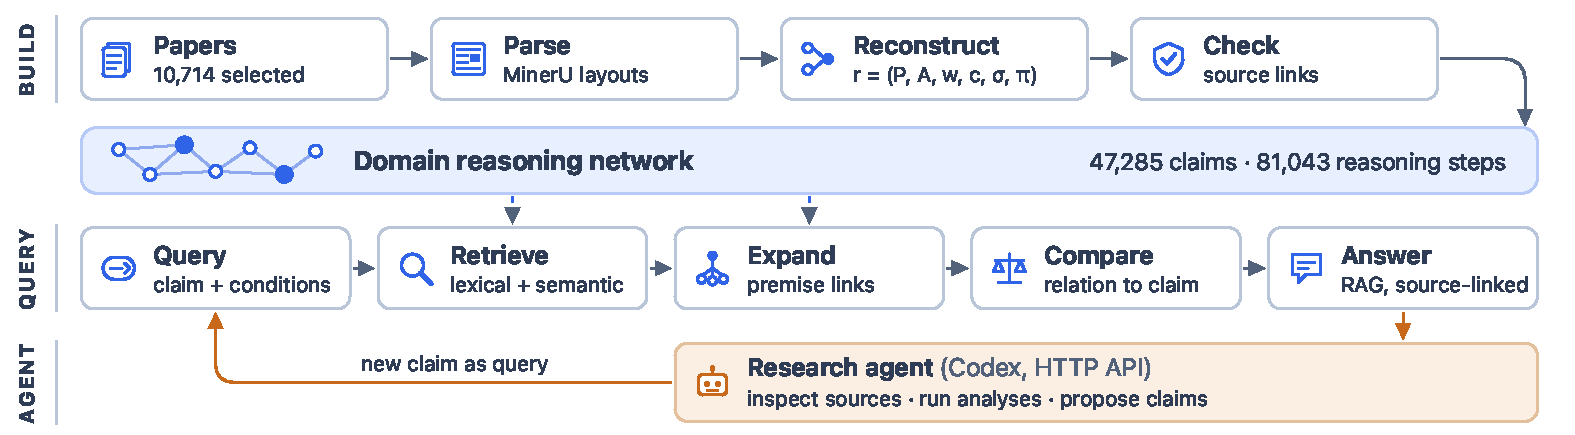
\includegraphics[width=\textwidth,trim=0 3pt 0 3pt,clip]{figures/system-architecture.pdf}
\caption{DeepShovel 2.0 architecture. Papers form a source-linked reasoning network for claim verification; agent-proposed claims return as queries.}
\Description{The build pipeline creates a domain reasoning network. The query pipeline retrieves, expands, and compares arguments. A research agent inspects sources, runs analyses, and returns new claims to the query pipeline.}
\label{fig:system-overview}
\end{figure*}

\section{Introduction}
Scientific conclusions depend on observations, assumptions, and inferential steps. To reuse a conclusion, researchers need to understand its evidence and limits. We illustrate these needs by checking the assumptions behind a fault-pressure estimate and testing whether a seawater-pH predictor transfers to new observations.

\sys{} represents a reusable scientific argument as a conclusion together with its premises, assumptions, reasoning steps, and source links. It reconstructs each selected paper's research question, main claims, and inferential dependencies, then connects these arguments across selected domain literature. The network records when each conclusion applies and how it supports, qualifies, or challenges other conclusions. It supports two complementary operations: tracing a conclusion backward to its justification, and using source-supported premises to derive new, testable claims.

To make arguments traceable across scholarly resources, each reasoning step links to specific documents, passages, figures, tables, and data. Users follow these links from a generated answer to its argument and original evidence. The application, walkthrough, evaluation data, and research package are available at \url{https://github.com/spiderLL2002/deepshovel-www2027}.

\paragraph{Contribution and positioning.}
GeoDeepShovel builds scientific databases from literature~\cite{geodeepshovel}. DeepShovel~2.0 extends literature reuse to the arguments connecting data, assumptions, and conclusions. Related work addresses claim verification with evidence rationales~\cite{scifact}, inter-document argument relations~\cite{argumentweb}, and graph-based synthesis~\cite{graphrag}. ResearchAgent~\cite{researchagent} and DeepEvidence~\cite{deepevidence} extend literature use toward iterative idea generation and evidence exploration. DeepShovel connects these tasks in three ways. First, each inference node links the premises and assumptions used together in one reasoning step to its conclusion. Second, the system checks whether these premises support the target claim under the user's conditions. Third, agent-proposed claims re-enter the same evidence-search and comparison process. Figure~\ref{fig:architecture} illustrates condition checking through the friction, cohesion, and stress assumptions behind a pressure estimate.

\begin{figure*}[t]
\centering
\begin{minipage}[t]{0.48\textwidth}
\vspace{0pt}
{\sffamily\footnotesize\bfseries\color{navy}(a) Live claim inspector}\par
\smallskip{\color{navy!25}\hrule height .45pt}\smallskip
\centering\resizebox*{!}{134pt}{\begin{minipage}{\linewidth}
\noindent
\includegraphics[width=\linewidth]{../artifact/live-demo/en-f2-claim.png}\par\vspace{2pt}
\noindent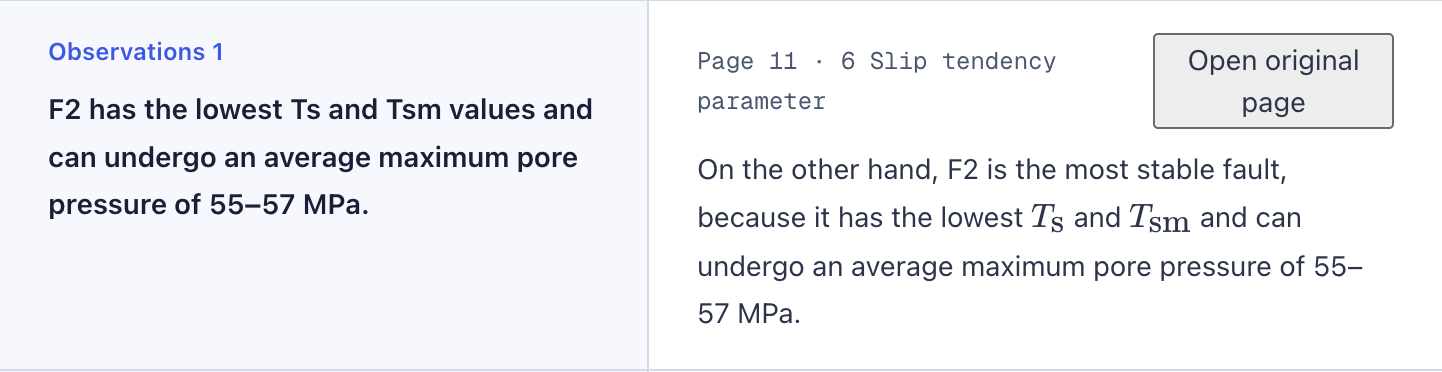
\includegraphics[width=\linewidth]{../artifact/live-demo/en-f2-source.png}\par\vspace{2pt}
\noindent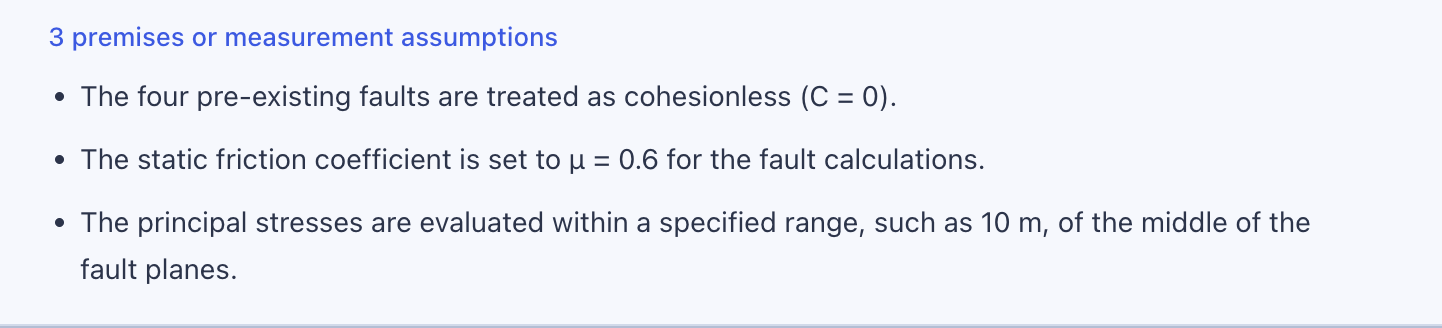
\includegraphics[width=\linewidth]{../artifact/live-demo/en-f2-assumptions.png}
\end{minipage}}
\end{minipage}\hfill
\begin{minipage}[t]{0.49\textwidth}
\vspace{0pt}
{\sffamily\footnotesize\bfseries\color{navy}(b) Dependencies and condition check}\par
\smallskip{\color{navy!25}\hrule height .45pt}\smallskip
\centering
\resizebox*{!}{134pt}{%
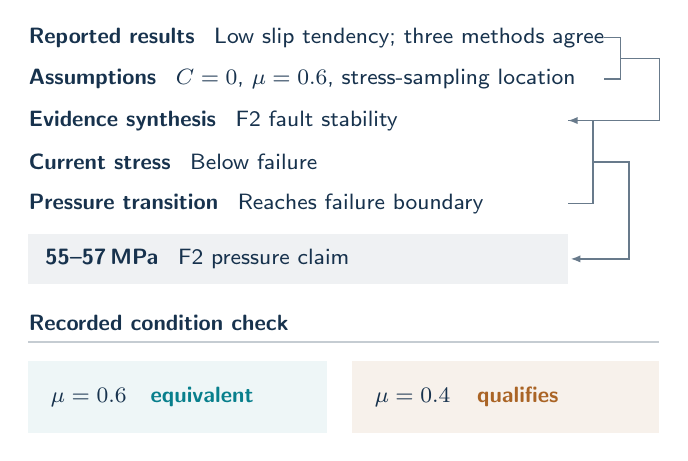
\begin{tikzpicture}[x=1pt,y=1pt,font=\sffamily\footnotesize,
  labeltext/.style={anchor=west,inner sep=0pt,text=navy},
  dependency/.style={draw=navy!65,line width=.55pt}]
\node[labeltext] at (0,-5) {\textbf{Reported results} \enspace Low slip tendency; three methods agree};
\node[labeltext] at (0,-20) {\textbf{Assumptions} \enspace $C=0$, $\mu=0.6$, stress-sampling location};
\draw[dependency] (208,-5) -- (214,-5) -- (214,-20) -- (208,-20);
\draw[dependency,-{Latex[length=3.5pt]}] (214,-12.5) -- (228,-12.5) |- (204,-35) -- (195,-35);
\node[labeltext] at (0,-35) {\textbf{Evidence synthesis} \enspace F2 fault stability};
\node[labeltext] at (0,-50) {\textbf{Current stress} \enspace Below failure};
\node[labeltext] at (0,-65) {\textbf{Pressure transition} \enspace Reaches failure boundary};
\draw[dependency] (195,-35) -- (204,-35) -- (204,-65) -- (195,-65);
\draw[dependency,-{Latex[length=3.5pt]}] (204,-50) -- (217,-50) |- (204,-85) -- (196,-85);
\fill[navy!7] (0,-94) rectangle (195,-76);
\node[labeltext] at (6,-85) {\textbf{55--57\,MPa} \enspace F2 pressure claim};
\node[labeltext,font=\sffamily\footnotesize\bfseries] at (0,-108) {Recorded condition check};
\draw[navy!25,line width=.45pt] (0,-115) -- (228,-115);
\fill[teal!7] (0,-148) rectangle (108,-122);
\fill[amber!9] (117,-148) rectangle (228,-122);
\node[labeltext] at (8,-135) {$\mu=0.6$};
\node[labeltext,text=teal,font=\sffamily\footnotesize\bfseries] at (44,-135) {equivalent};
\node[labeltext] at (125,-135) {$\mu=0.4$};
\node[labeltext,text=amber,font=\sffamily\footnotesize\bfseries] at (162,-135) {qualifies};
\end{tikzpicture}}
\end{minipage}
\caption{F2 condition checking. (a) Live claim, source, and assumptions. (b) Recorded inference inputs and comparison outcomes for two friction coefficients. The full argument contains 18 premise links.}
\Description{A live screenshot shows the 55--57 MPa claim, its original passage, and three assumptions. Joint inputs lead to the pressure estimate. The condition check returns equivalence at a friction coefficient of 0.6 and qualification at 0.4.}
\label{fig:architecture}
\end{figure*}

\section{Building a Domain Reasoning Network}
\label{sec:network}
The system first parses papers and reconstructs their arguments. At query time, it retrieves candidate claims, expands their recorded dependencies, and compares the resulting arguments with the target claim. The browser exposes claims, their reasoning, and original evidence (Figure~\ref{fig:architecture}); an external agent orchestrates further source inspection and analysis (Section~\ref{sec:agents}).
\paragraph{Running system.}
With guidance from domain experts, we selected 10,714 papers on ocean anoxia and deep-sea rare earth elements from a corpus of 1,401,532 parsed geoscience publications. The resulting DeepShovel 2.0 library contains 47,285 claims and 81,043 reasoning steps. MinerU parses document layouts; current reconstruction and comparison use GPT-6-Luna. A curation interface supports paper selection and source-linked review. Queries compare up to 50 candidates and follow recorded dependencies to a maximum depth of 32.
\paragraph{Reconstruct the paper's reasoning.}
The parser extracts passages, equations, tables, figure panels, and supplementary data, recording their locations in the original document. Reconstruction follows the paper's main reasoning routes: question $\rightarrow$ methods and assumptions $\rightarrow$ observations $\rightarrow$ intermediate interpretations $\rightarrow$ conclusions. Users trace a conclusion backward to its observations and assumptions, or follow observations forward through intermediate interpretations to final claims.

\begin{samepage}
We represent each reasoning step as
\begin{equation}
r=(P_r,A_r,w_r,c_r,\sigma_r,\pi_r).
\end{equation}
Here, $P_r$ lists observations and intermediate findings used together in the step. $A_r$ lists its assumptions, and $w_r$ describes in natural language how these inputs support conclusion $c_r$. The fields $\sigma_r$ and $\pi_r$ record applicability conditions and source locations. An assumption states what a derivation takes as given; an applicability condition records where its conclusion can be used. For example, a friction assumption also restricts the pressure claim to that modeled setting. Each inference node represents one reasoning step and groups the premises and assumptions used together to support its conclusion. Alternative derivations of the same conclusion occupy separate inference nodes. When a claim is opened, the system follows its stored links to retrieve the premises and assumptions used in each supporting step.
\end{samepage}

For fault F2 in the Asmari reservoir~\cite{asmari}, the argument combines two reported analysis results---fault stability and agreement among three methods---with three assumptions (Figure~\ref{fig:architecture}). Current-stress analysis sets the initial state. Critical-pressure analysis then estimates when rising pore pressure would bring the fault to the modeled failure boundary. Users can inspect both the analysis and its original source.

Each reasoning step retains its applicability conditions and source locations. Conditions cover material, setting, method, comparator, and temporal or spatial range. Reconstruction distinguishes observations, interpretations, and predictions and retains quantifiers and negation. Source links identify a document version and a passage, equation, table, figure panel, or dataset record. Values retain units and uncertainty; figures retain captions and experimental context. Source passages remain accessible alongside reconstructed reasoning and agent proposals.

\paragraph{Connect arguments across papers.}
The same representation connects claims across papers while retaining their separate arguments and sources. For ecosystem-collapse timing at Fiskegrav, the system retrieves van Soelen et al.'s~\cite{fiskegravduration} 1.6--8 kyr estimate. It also returns Mettam et al.'s~\cite{fiskegravevent} evidence of continued animal disturbance of sediments after the last macrofossil. This supplementary argument distinguishes the disappearance of macrofossils from final ecosystem collapse. Users open both source pages to check which event the duration describes.


\paragraph{Model tasks and programmatic checks.}
Language models reconstruct reasoning steps and compare claims in context. Programmatic checks validate source identifiers and references; dependency traversal follows the stored links. This division connects source-grounded reconstruction with the query-time comparison described next.

\section{Reasoning-Level Retrieval and Verification}
\label{sec:verification}
\paragraph{Retrieve the justification of an answer.}
For each query, the system identifies the target claim, its applicability conditions, and the evidence needed to assess it. Lexical and semantic search retrieve candidate claims and observations. Dependency traversal then collects each candidate's premises, assumptions, and source evidence into an \emph{expanded argument}. A single model call uses these arguments to rank candidates and assign their relations to the target claim. Support and counterevidence searches cover incompatible observations, alternative mechanisms, failed transfers, and challenged assumptions.

During comparison, the search list displays a preview. The final relations distinguish equivalent conclusions from results that hold under different conditions. Users inspect the same expanded arguments and follow individual premises to their original pages.

After comparison, retrieval-augmented generation (RAG) produces an answer with explicit applicability conditions and links its assertions to reasoning steps and evidence.

\paragraph{Locate the disagreement inside the argument.}
Verification distinguishes equivalent claims, supporting evidence, contradictions, qualifications, and related evidence. Equivalence requires the same proposition under compatible conditions; a qualification limits where the result applies. A counterexample must address the claimed scope; evidence from another setting may instead challenge a generalization. The system identifies whether the disagreement concerns an observation, an assumption, or an inference. Dependency traversal connects principal claims; cross-paper alignment exposes differences in data, methods, or applicability.

\paragraph{Retrieval evaluation.}
We compare BM25, dense retrieval, reciprocal rank fusion, and hybrid retrieval on 430 geoscience questions with 12,541 reference judgments. A complete answer appears in the top three for 399/430 hybrid queries (92.79\%) and 393/430 BM25 queries (91.40\%). Counting complete or partial answers gives 421/430 (97.91\%) and 415/430 (96.51\%), respectively. On the 119 questions with fully judged candidate pools, nDCG@10 is 0.842 for hybrid and 0.859 for BM25. The nDCG pools include supplementary AI judgments.

\paragraph{Argument comparison.}
The test comprises 264 cases from 65 papers. Two domain experts independently reviewed the source passages and identified acceptable relations. A third adjudicated disagreements. The 79 development cases come from 17 different papers. The query, candidate, prompt, and model settings are fixed across representations. GPT-6-Luna is the primary model, with DeepSeek V4 Flash available as fallback. The flat argument retains the nodes and text but removes dependency edges and anchor references. The final run counts predictions matching an accepted relation from candidate to query.
\par{\centering\small
\begin{tabular}{@{}lr@{}}
\toprule
Comparison input & Correct / total\\
\midrule
Claim and conditions & 217/264\\
Expanded argument & 241/264\\
Source passages & 221/264\\
Flat argument & 229/264\\
\bottomrule
\end{tabular}
\par}
The final end-to-end run matched relation and direction for 79/87 queries in group~A and 73/88 in group~B. The denominators include zero and zero failed queries, respectively. Mean times for completed queries were 40.99 and 40.74 seconds. A source audit found full support for 129/129 scientific nodes and 120/124 dependencies. The other four dependencies were partially supported.

\paragraph{Interactive condition check.}
For F2, a user opens the 55--57\,MPa pressure claim and inspects the zero-cohesion, friction, and stress-sampling assumptions (Figure~\ref{fig:architecture}). The system retrieves all three recorded assumptions for comparison. The recorded condition check returned equivalence at $\mu=0.6$ and qualification at $\mu=0.4$. The source estimate requires friction $\mu=0.6$ (page~11~\cite{asmari}).

\begin{figure*}[t]
\centering
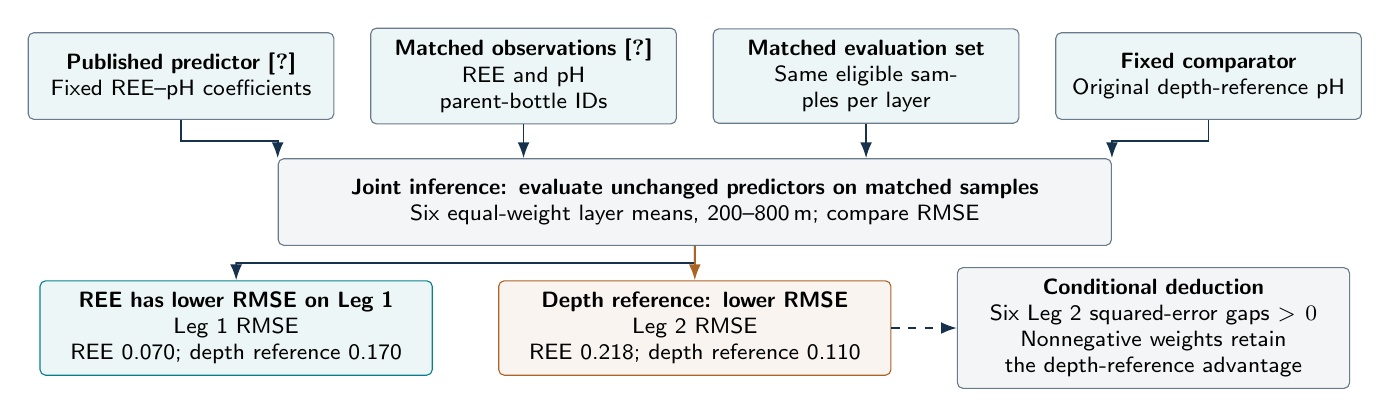
\begin{tikzpicture}[font=\sffamily\footnotesize,>=Latex,
nodebox/.style={draw=navy!65,rounded corners=2pt,align=center,inner sep=4pt,minimum height=11mm},
arr/.style={->,draw=navy,semithick}]
\node[nodebox,fill=pale,text width=36mm] (m) at (0,0) {\textbf{Published predictor~\cite{lin2024}}\\Fixed REE--pH coefficients};
\node[nodebox,fill=pale,text width=36mm] (d) at (4.35,0) {\textbf{Matched observations~\cite{gp15}}\\REE and pH parent-bottle IDs};
\node[nodebox,fill=pale,text width=36mm] (s) at (8.7,0) {\textbf{Matched evaluation set}\\Same eligible samples per layer};
\node[nodebox,fill=pale,text width=36mm] (b) at (13.05,0) {\textbf{Fixed comparator}\\Original depth-reference pH};
\node[nodebox,fill=navy!5,text width=103mm] (r) at (6.525,-1.6) {\textbf{Joint inference: evaluate unchanged predictors on matched samples}\\Six equal-weight layer means, 200--800\,m; compare RMSE};
\coordinate (inputjoin) at ($(d.south)!0.5!(r.north)$);
\draw[arr] (m.south)--(m.south |- inputjoin)-|(r.north west);
\draw[arr] (d.south)--(r.north -| d.south);
\draw[arr] (s.south)--(r.north -| s.south);
\draw[arr] (b.south)--(b.south |- inputjoin)-|(r.north east);
\node[nodebox,draw=teal,fill=pale,text width=47mm] (a) at (0.7,-3.2) {\textbf{REE has lower RMSE on Leg 1}\\Leg 1 RMSE\\REE 0.070; depth reference 0.170};
\node[nodebox,draw=amber,fill=amber!7,text width=47mm] (c) at (6.525,-3.2) {\textbf{Depth reference: lower RMSE}\\Leg 2 RMSE\\REE 0.218; depth reference 0.110};
\node[nodebox,fill=navy!5,text width=47mm] (h) at (12.35,-3.2) {\textbf{Conditional deduction}\\Six Leg 2 squared-error gaps $>0$\\Nonnegative weights retain\\the depth-reference advantage};
\coordinate (outputjoin) at ($(r.south)!0.5!(c.north)$);
\draw[arr] (r.south)--(outputjoin)-|(a.north);
\draw[arr,draw=amber] (r.south)--(c.north);
\draw[arr,dashed] (c.east)--(h.west);
\end{tikzpicture}
\caption{GP15 argument. Four joint premises support the comparison; the dashed arrow adds the six layerwise error checks underlying the conditional reweighting claim.}
\Description{Four joint premises feed a fixed-model comparison: original coefficients, matched observations, common sampling support, and a fixed depth reference. A favorable branch retains local support, an adverse branch challenges transfer, and a dashed arrow marks a scoped deduction about arbitrary nonnegative depth weights.}
\label{fig:argument}
\end{figure*}




\section{Agent-Guided Discovery and Workflow Refinement}
\label{sec:agents}
An agent starts with a retrieved argument and uses its premises to formulate a testable extension. DeepShovel supplies the source-linked arguments and comparisons, while Codex coordinates source inspection, numerical analysis, and a record of candidate claims, their evidence, and their status. Codex accesses search and argument graphs through DeepShovel's HTTP API, then submits proposed claims as queries for counterevidence and prior work. We use task-level recursive self-improvement (RSI) for the agent's feedback-driven revision of its investigation protocol: the revised rule is saved and checked in the next analysis run.

\paragraph{An executed geoscience investigation.}
Across eight rounds, Codex screened 48 research questions for source support, novelty, and executable analyses. The selected study tested a published seawater-pH calibration~\cite{lin2024} on two GP15 station groups. The calibration predicts pH from the slope of shale-normalized concentrations of four rare-earth elements: Sm, Gd, Dy, and Er.

DeepShovel supplied this rare-earth-element (REE) calibration argument and source; Codex defined a fixed-model test with public observations from the GEOTRACES GP15 Pacific transect~\cite{gp15}. REE and pH measurements were matched by parent-bottle identifiers, retaining their filtration status. The REE--pH predictor was compared with a depth reference based on the original calibration notebook. Both were evaluated against total-scale pH at 25$^\circ$C and surface pressure, using the same eligible samples in six 100-m layers from 200 to 800\,m. The depth reference uses the global pH mean for each layer saved in the original calibration notebook; neither predictor was refitted. The reported RMSE compares layer-mean predictions with layer-mean observations across the six layers. This comparison favored REE on Leg~1 and the depth reference on Leg~2 (Table~\ref{tab:case}). Within 200--800\,m, the REE predictor therefore had higher RMSE on Leg~2. Figure~\ref{fig:argument} shows the data-matching and evaluation choices supporting this comparison.



\begin{table}[b]
\caption{GP15 RMSE (pH units) across six equal-weight layer means. Leg~1: Seattle--Hilo; Leg~2: Hilo--Papeete. Both methods use identical eligible samples per layer.}
\label{tab:case}
\centering
\begin{tabular}{@{}lrrr@{}}
\toprule
GP15 group & Bottles / stations & REE model & Depth reference\\
\midrule
Leg 1 & 24 / 6 & 0.070 & 0.170\\
Leg 2 & 55 / 8 & 0.218 & 0.110\\
\bottomrule
\end{tabular}
\end{table}

The agent then derived a new conditional claim from the layerwise errors. For each of the six Leg~2 layers, the squared error of the REE predictor exceeded that of the depth reference. \mbox{Let $d_i=e_{\mathrm{REE},i}^2-e_{\mathrm{ref},i}^2$.} All six differences are positive, with a minimum of 0.00545\,pH$^2$. Therefore, $\sum_i w_i d_i>0$ for any shared nonnegative weights summing to one: no shared nonnegative weighting of these six fixed layer means can reverse the depth reference's lower RMSE.

Codex records the comparison and deduction as distinct claims with data and analysis links. Codex queries each claim and its conditions for supporting evidence or competing explanations.

The GP15 study also illustrates task-level RSI. Agent review checked a revised rule for reporting station-bootstrap intervals: at least six original stations and all six depth layers in at least 90\% of resamples. Codex saved and reran the protocol; 97.5\% and 97.8\% of resamples retained all six layers for Legs~1 and~2.

\section{Interactive Demonstration}
\label{sec:demo}
The demo follows three questions: What supports this conclusion? Does it apply here? What can we infer next?

\paragraph{1. Understand a published conclusion.}
Attendees enter the F2 pressure claim and open its source paper. They expand its observations, reasoning steps, and three assumptions, then open the original passage on page~11 (Figure~\ref{fig:architecture}).

\paragraph{2. Examine support and disagreement.}
Next, attendees change a condition in their target claim, such as the assumed friction coefficient for F2, or request counterevidence. The comparison assesses whether the recorded premises support this revised claim and presents the relation with its evidence. They follow each result through its premises to examine its applicability.

\paragraph{3. Extend the investigation with an agent.}
Finally, attendees follow the completed GP15 study from its research question to the comparison and conditional deduction in Figure~\ref{fig:argument}. Using the configured Codex session, attendees can then propose another station group or request literature that could challenge the inference. During the live demo, a new request runs the initial literature search and planning steps. The saved GP15 study provides immediate access to the later analyses and recorded claims.

\paragraph{Conference setup and public materials.}
A laptop runs the configured application and a Codex session. Fresh model requests require network access. The repository includes the English walkthrough, source pages, and the ten-stage GP15 analysis, which reproduced 76 files byte for byte in the reference environment.

\section{Ethical Use of Data}
Publications and data are used under their licenses, with attribution, source versions, and provenance retained. The GP15 study reanalyzes public measurements.

\begin{thebibliography}{10}
\bibitem{geodeepshovel}
Shao Zhang et al. 2023. GeoDeepShovel: A platform for building scientific database from geoscience literature with AI assistance. \emph{Geoscience Data Journal} 10, 4, 519--537. \url{https://doi.org/10.1002/gdj3.186}
\bibitem{scifact}
David Wadden et al. 2020. Fact or Fiction: Verifying Scientific Claims. In \emph{EMNLP}, 7534--7550. \url{https://doi.org/10.18653/v1/2020.emnlp-main.609}
\bibitem{argumentweb}
Florian Ruosch, Cristina Sarasua, and Abraham Bernstein. 2025. Mining Inter-Document Argument Structures in Scientific Papers for an Argument Web. \emph{Transactions on Graph Data and Knowledge} 3, 3, Article 4. \url{https://doi.org/10.4230/TGDK.3.3.4}
\bibitem{graphrag}
Darren Edge et al. 2024. From Local to Global: A Graph RAG Approach to Query-Focused Summarization. \emph{arXiv:2404.16130}. \url{https://arxiv.org/abs/2404.16130}
\bibitem{researchagent}
Jinheon Baek, Sujay Kumar Jauhar, Silviu Cucerzan, and Sung Ju Hwang. 2025. ResearchAgent: Iterative Research Idea Generation over Scientific Literature with Large Language Models. In \emph{NAACL}, 6709--6738. \url{https://doi.org/10.18653/v1/2025.naacl-long.342}
\bibitem{deepevidence}
Zifeng Wang et al. 2026. Empowering biomedical evidence exploration and synthesis with deep knowledge graph research. \emph{Nature Machine Intelligence} 8, 1142--1156. \url{https://doi.org/10.1038/s42256-026-01266-0}
\bibitem{lin2024}
Ping-Chun Lin and David C. Catling. 2024. The Rare Earth Element Distribution in Marine Carbonates as a Potential Proxy for Seawater pH on Early Earth. \emph{American Journal of Science} 324, Article 10. \url{https://doi.org/10.2475/001c.118215}
\bibitem{gp15}
BCO-DMO. GEOTRACES GP15 rare earth element and pH datasets. REE: \url{https://doi.org/10.26008/1912/bco-dmo.932161.1}, \url{https://doi.org/10.26008/1912/bco-dmo.932559.1}; pH: \url{https://doi.org/10.26008/1912/bco-dmo.838157.2}, \url{https://doi.org/10.26008/1912/bco-dmo.838173.2}.
\bibitem{asmari}
Majid Taghipour et al. 2019. Estimation of the current stress field and fault reactivation analysis in the Asmari reservoir, SW Iran. \emph{Petroleum Science} 16, 513--526. \url{https://doi.org/10.1007/s12182-019-0331-9}
\bibitem{fiskegravduration}
Elsbeth E. van Soelen et al. 2018. Salinity changes and anoxia resulting from enhanced run-off during the late Permian global warming and mass extinction event. \emph{Climate of the Past} 14, 441--453. \url{https://doi.org/10.5194/cp-14-441-2018}
\bibitem{fiskegravevent}
C. Mettam et al. 2017. High-frequency fluctuations in redox conditions during the latest Permian mass extinction. \emph{Palaeogeography, Palaeoclimatology, Palaeoecology} 485, 210--223. \url{https://doi.org/10.1016/j.palaeo.2017.06.014}
\end{thebibliography}
\end{document}
